%==============================================================

\section{Big Data Framework Spark}\label{bds1}

After the features are extracted, the next step is to load the feature files into the HDFS. 
The first tests with spark were performed on a single PC with 4 CPU cores, running Spark 2.4.0.\\ The cluster test were performed on the ARA- Cluster, that offers 16 compute-nodes with 32 CPU-cores per node (72 with HT) and 192GB RAM. The cluster was running an older version of Spark (1.6.0)\\

\subsection{Data preprocessing}

The features are stored in text files as described in chapter \ref{sumfeat}. Due to the fact that the features were extracted in parallel and in batches of only a few songs, each of the feature files only contain the features of a small number of songs. Because many small files are inefficient to process with Spark \cite[p. 153]{sparkbook1} all files containing the same feature type are merged to one large file, before being loaded into the HDFS. By loading larger files into the HDFS, the partitioning into data blocks is performed according to the standard parameters of the HDFS (e.g. 128 MB partitions). Additional repartitioning on the cluster is later performed with Spark by using the \textit{rdd.coalesce(repartition\_count)} command. 
Finally to work with the features a few transformations have to be performed on the data. For example the extracted note values are stored as lists of numbers, each representing a certain note. To compare these using the Levenshtein distance, these lists are converted into strings. 

\begin{pythonCode}
chroma = sc.textFile("features/out[0-9]*.notes").coalesce(repartition_count)
chroma = chroma.map(lambda x: x.split(';'))
chroma = chroma.map(lambda x: (x[0], x[1], x[2], x[3].replace("0",'A').replace("1",'B').replace("2",'C').replace("3",'D').replace("4",'E').replace("5",'F').replace("6",'G').replace("7",'H').replace("8",'I').replace("9",'J').replace("10",'K').replace("11",'L')))
chroma = chroma.map(lambda x: (x[0], x[1], x[2], x[3].replace(',','').replace(' ','')))
df = spark.createDataFrame(chroma, ["id", "key", "scale", "notes"])
\end{pythonCode}

All the other features are stored as lists of floats and have to be converted to vectors.  

\begin{pythonCode}
list_to_vector_udf = udf(lambda l: Vectors.dense(l), VectorUDT())
rp = sc.textFile("features[0-9]*/out[0-9]*.rp").coalesce(repartition_count)
rp = rp.map(lambda x: x.split(","))
kv_rp= rp.map(lambda x: (x[0].replace(";","").replace(".","").replace(",","").replace(" ",""), list(x[1:])))
rp_df = spark.createDataFrame(kv_rp, ["id", "rp"])
rp_df = rp_df.select(rp_df["id"],list_to_vector_udf(rp_df["rp"]).alias("rp"))
\end{pythonCode}

\subsection{Euclidean Distance}

\begin{pythonCode}
from scipy.spatial import distance
#...
distance_udf = F.udf(lambda x: float(distance.euclidean(x, comparator_value)), FloatType())
result = df_vec.withColumn('distances', distance_udf(F.col('features')))
result = result.select("id", "distances").orderBy('distances', ascending=True)
result = result.rdd.flatMap(list).collect()
\end{pythonCode}

\noindent\textit{\textbf{Explain usage of user defined function udf\\}}
\ \\
\noindent\textit{\textbf{Used with BH, RH, BP AND MFCC\\}}
\ \\
\noindent\textit{\textbf{super versatile AND very fast\\}}
\ \\
\noindent\textit{\textbf{insert analysis of performance\\}}

\subsection{Bucketed Random Projection}

Due to the fact that the ARA cluster is running with PySpark version 1.6.0, the Bucketed Random Projection (BRP) Algorithm could only be tested on the single node test platform. 

\begin{pythonCode}
from pyspark.ml.feature import BucketedRandomProjectionLSH
#...
brp = BucketedRandomProjectionLSH(inputCol="features", outputCol="hashes", seed=12345, bucketLength=25.0)
model = brp.fit(df_vec)
comparator_value = Vectors.dense(comparator[0])
result = model.approxNearestNeighbors(df_vec, comparator_value, df_vec.count()).collect()
rf = spark.createDataFrame(result)
result = rf.select("id", "distCol").rdd.flatMap(list).collect()
\end{pythonCode}

\noindent\textit{\textbf{Usable as a substitute for euclidean UDF\\}}
\ \\
\noindent\textit{\textbf{Is it faster than the UDF tho? - performance test\\}}

\subsection{Cross-correlation}

\FloatBarrier
\begin{figure}[htbp]
	\centering
	\framebox{\parbox{1\textwidth}{
			\begin{subfigure}{.495\textwidth}
				\centering
				\includegraphics[scale=0.22]{Images/Spark/df_slow_chroma.png}
				\caption{Chroma multiple agg}
				\label{chr2}
			\end{subfigure}%
			
			\begin{subfigure}{.495\textwidth}
				\centering
				\includegraphics[scale=0.22]{Images/Spark/df_speed_chroma.png}
				\caption{Chroma single agg}
				\label{chr1}
			\end{subfigure}% 	
			
			\begin{subfigure}{.495\textwidth}
				\centering
				\includegraphics[scale=0.22]{Images/Spark/toPandasDag.png}
				\caption{DAG toPandas}
				\label{chr3}
			\end{subfigure}% 		
	}}
	\caption{Chroma on 11500 songs, single node}
	\label{fig:chroma}
\end{figure}
\FloatBarrier

\textit{\textbf{2 Versions explained - with additional key shift and without}}
\begin{pythonCode}
def cross_correlate(chroma1, chroma2):
    corr = sp.signal.correlate2d(chroma1, chroma2, mode='full')
    #transposed_chroma = transposed_chroma / (min(length1, length2))
    index = np.where(transposed_chroma == np.amax(transposed_chroma))
    index = int(index[0])
    mean_line = transposed_chroma[index]
    sos = sp.signal.butter(1, 0.1, 'high', analog=False, output='sos')
    mean_line = sp.signal.sosfilt(sos, mean_line)
    return np.max(mean_line)
#...
distance_udf = F.udf(lambda x: float(cross_correlate(x, comparator_value)), DoubleType())
result = df_vec.withColumn('distances', distance_udf(F.col('chroma')))
result = result.select("id", "distances").orderBy('distances', ascending=False)
result = result.rdd.flatMap(list).collect()
\end{pythonCode}

\noindent\textbf{\textit{Memory intense - had to alter spark-defaults.conf\\}}
\textit{spark.driver.memory             6g\\
spark.executor.memory           2g\\
}
\noindent\textbf{\textit{Insert graphics of calculation time with and without correlation\\}}
\ \\
\noindent\textbf{\textit{Differences in the results to the original paper can be explained with the different underlying beat tracking, different filter parameters and a few improvements that are left out as mentioned in \ref{chromafeat}}\cite{cover802}}

\subsection{Kullback-Leibler Divergence}

\begin{pythonCode}
def symmetric_kullback_leibler(vec1, vec2):
	#preprocessing: splitting vec1 and vec2 into mean1, mean2, cov1 and cov2
    d = 13
    div = 0.25 * (np.trace(cov1 * np.linalg.inv(cov2)) + np.trace(cov2 * np.linalg.inv(cov1)) + np.trace( (np.linalg.inv(cov1) + np.linalg.inv(cov2)) * (mean1 - mean2)**2) - 2*d)
    return div
distance_udf = F.udf(lambda x: float(symmetric_kullback_leibler(x, comparator_value)), DoubleType())
result = df_vec.withColumn('distances', distance_udf(F.col('features')))
result = result.select("id", "distances").orderBy('distances', ascending=True)
result = result.rdd.flatMap(list).collect()
\end{pythonCode}

\noindent\textbf{\textit{Differences in the results to the original musly tool can be explained due to the choice of only 13 MFCC bands in this thesis compared to the 25 bands in musly}\cite{musly1}}

\subsection{Jensen-Shannon Divergence}

\begin{pythonCode}
def jensen_shannon(vec1, vec2):
	#preprocessing: splitting vec1 and vec2 into mean1, mean2, cov1 and cov2
    mean_m = 0.5 * (mean1 + mean2)
    cov_m = 0.5 * (cov1 + mean1 * np.transpose(mean1)) + 0.5 * (cov2 + mean2 * np.transpose(mean2)) - (mean_m * np.transpose(mean_m))
    div = 0.5 * np.log(np.linalg.det(cov_m)) - 0.25 * np.log(np.linalg.det(cov1)) - 0.25 * np.log(np.linalg.det(cov2))  
    if np.isnan(div):
        div = np.inf
    return div
distance_udf = F.udf(lambda x: float(jensen_shannon(x, comparator_value)), DoubleType())
result = df_vec.withColumn('distances', distance_udf(F.col('features')))
result = result.select("id", "distances").orderBy('distances', ascending=True)
result = result.rdd.flatMap(list).collect()
\end{pythonCode}

\noindent\textbf{\textit{Problem mit den "skyrocketing determinanten" -> Lösung: cholesky zerlegung, geht nicht - nicht positiv definit, Lösung 2 nutzen von SKL aber noch rechenintensiver!}\cite[p.45]{schnitzer1}}

\subsection{Levenshtein distance}

\begin{pythonCode}
def get_neighbors_notes(song):
    filterDF = df.filter(df.id == song)
    filterDF.first()
    comparator_value = filterDF.collect()[0][3] 
    print comparator_value
    df_merged = df.withColumn("compare", lit(comparator_value))
    df_levenshtein = df_merged.withColumn("word1_word2_levenshtein", levenshtein(col("notes"), col("compare")))
    df_levenshtein.sort(col("word1_word2_levenshtein").asc()).show()
\end{pythonCode}

\subsection{performance}

\begin{pythonCode}
confCluster = SparkConf().setAppName("MusicSimilarity Cluster")
confCluster.set("spark.driver.memory", "64g")
confCluster.set("spark.executor.memory", "64g")
confCluster.set("spark.driver.memoryOverhead", "32g")
confCluster.set("spark.executor.memoryOverhead", "32g")
#Be sure that the sum of the driver or executor memory plus the driver or executor memory overhead is always less than the value of yarn.nodemanager.resource.memory-mb
#confCluster.set("yarn.nodemanager.resource.memory-mb", "192000")
#spark.driver/executor.memory + spark.driver/executor.memoryOverhead < yarn.nodemanager.resource.memory-mb
confCluster.set("spark.yarn.executor.memoryOverhead", "4096")
#set cores of each executor and the driver -> less than avail -> more executors spawn
confCluster.set("spark.driver.cores", "32")
confCluster.set("spark.executor.cores", "32")
confCluster.set("spark.dynamicAllocation.enabled", "True")
confCluster.set("spark.dynamicAllocation.minExecutors", "16")
confCluster.set("spark.dynamicAllocation.maxExecutors", "32")
confCluster.set("yarn.nodemanager.vmem-check-enabled", "false")
repartition_count = 32
\end{pythonCode}

\subsubsection{Differences between the feature types}


\subsubsection{Performance Comparison of RDD vs DataFrames vs single DataFrame}

\noindent\textbf{\textit{Explain Single DataFrame vs multiple DataFrames}}

\FloatBarrier
\begin{figure}[htbp]
	\centering
	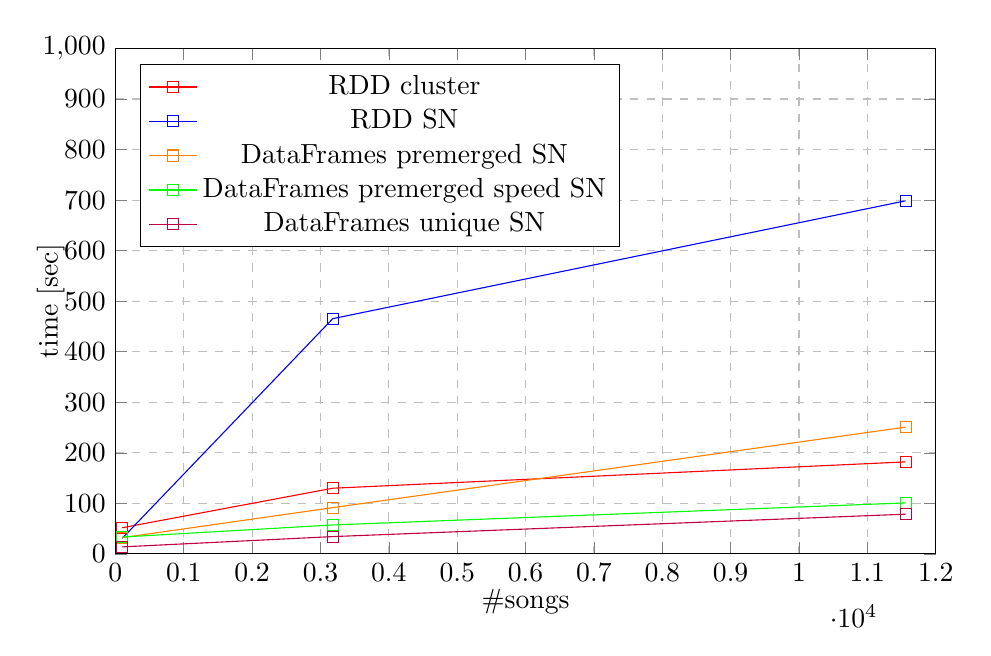
\begin{tikzpicture}
	\centering
	\begin{axis}[
	    %title={Performance of various toolkits},
		x label style={at={(axis description cs:0.5,-0.05)},anchor=north},
		y label style={at={(axis description cs:-0.05,.5)},rotate=0,anchor=south},
	    xlabel={\#songs},
	    ylabel={time [sec]},
	    xmin=0, xmax=12000,
	    ymin=0, ymax=1000,
	    xtick={0,1000,2000,3000,4000,5000,6000,7000,8000,9000,10000,11000,12000},
	    ytick={0,100,200,300,400,500,600,700,800,900,1000},
	    legend pos=north west,
	    ymajorgrids=true,
	    grid style=dashed,
	    height=8cm,
	    width=12cm,
	    grid=major,
	]
	\addplot[
		color=red,
		mark=square,
		]
		coordinates {
	    (100,51.736)(3180,129.940)(11560,182.035)
		};
		\addlegendentry{RDD cluster}
	\addplot[
	    color=blue,
	    mark=square,
	    ]
	    coordinates {
	    (100,30.770)(3180,465.445)(11560,698.657)
	    };
	    \addlegendentry{RDD SN}
	\addplot[
	    color=orange,
	    mark=square,
	    ]
	    coordinates {
	    (100,32.087)(3180,91.477)(11560,250.854)
	    };
	    \addlegendentry{DataFrames premerged SN}
	  
	\addplot[
	    color=green,
	    mark=square,
	    ]
	    coordinates {
	    (100,33.351)(3180,57.230)(11560,100.884)
	    };
	    \addlegendentry{DataFrames premerged speed SN}

	\addplot[
	    color=purple,
	    mark=square,
	    ]
	    coordinates {
	    (100,13.874)(3180,34.232)(11560,78.566)
	    };
	    \addlegendentry{DataFrames unique SN}	    
	\end{axis}
	\end{tikzpicture}
	\caption{Performance of various spark algorithms (MFCC Euc, Notes, RP)}
	\label{perfspark}
\end{figure}
\FloatBarrier


\subsubsection{min and max value aggregation}

\textit{\textbf{Why? Scaling of distances between 0 to 1 interval to combine different distances\\}}

\FloatBarrier
\begin{figure}[htbp]
	\centering
	\framebox{\parbox{1\textwidth}{
			\begin{subfigure}{.495\textwidth}
				\centering
				\includegraphics[scale=0.22]{Images/Spark/separate.png}
				\caption{Separate DataFrames}
				\label{sc3}
			\end{subfigure}%
			
			\begin{subfigure}{.495\textwidth}
				\centering
				\includegraphics[scale=0.22]{Images/Spark/df_merged.png}
				\caption{Single DataFrames, multiple collects}
				\label{sc4}
			\end{subfigure}% 	
			
			\begin{subfigure}{.495\textwidth}
				\centering
				\includegraphics[scale=0.22]{Images/Spark/speed_uo.png}
				\caption{Single DataFrames, single collects}
				\label{sc5}
			\end{subfigure}% 		
	}}
	\caption{Spark DF implementations, single node, 1517 artists}
	\label{fig:spark2}
\end{figure}
\FloatBarrier

\subsection{possible performance improvements}

\textit{\textbf{Pre- merge feature sets, broadcast comparator, descending importance pre-filtering\\}}
\\
\textit{\textbf{statistic normalization of similarities\\}}
\ \\
\textit{\textbf{Filter and refine after statistic normalization, drop all below mean\\}}
\ \\
\textit{\textbf{\underline{Is there a better way to cross-correlate???}\\}}
\ \\
\subsection{Other alternatives}

\subsubsection{Alternating Least Squares}

\subsubsection{TF-IDF weights}

\subsubsection{DIMSUM all-pairs similarity}